Los métodos no paramétricos se utilizan para estimar las funciones de densidad de probabilidad (f.d.p.) cuando no se conoce la expresión de la misma ni los parámetros.

\subsection{Esquema general}

Sea una cierta región R del espacio de características. La probabilidad $P_R$ de que un cierto x pertenezca a R viene dada por:

\[ P_R = p(x \in R) = \int_{R} p(x) dx \approx p(x) \int_{R} dx = p(x)*V \]

donde $V$ es el volumen ocupado por la región $R$.

Supongamos que disponemos de N muestras independientes $x_1
, x_2, ..., x_N$ correspondientes a la f.d.p. que queremos estimar, y dados:

\begin{itemize}
\item $k_N$ = cuántas de las N muestras pertenecen a la región R
\item $\frac{k_N}{N}$ es una estimación de $P_R$ para cada x, lo cual es a su vez una estimación de p(x).
\end{itemize}

Usando:
\[ p(x)*V \approx \frac{k_N}{N} \]

Podemos estimar $p(x)$ como :
\[ p(x) = \frac{\frac{k_N}{N}}{V} \]

Es decir, se aproxima $p(x)$ definiendo una región $R$ pequeña alrededor de x y contando cuántos de los $x_i$ caen en $R$.
En los ejercicios se aplicaron dos métodos no paramétricos: 

\begin{itemize}
\item Ventanas de Parzen
\item $k_{n}$ vecinos más cercanos
\end{itemize}

\subsection{Ventanas de Parzen}

Tomando una región $R$ con forma de hipercubo d-dimensional de lado $h_N$, entonces:

\[ V_N = (h_N)^d \]

Y sea la siguiente \textbf{función de ventana}:

\[ \varphi(x) = \left\{
\begin{array}{c l}
  1 & |u_j| \leq \frac{1}{2}, j=1..d \\
  0 & \text{caso contrario}
\end{array}
\right.
\]

Entonces, para un cierto x:

\[ \varphi(\frac{x-x_i}{h_N}) = 1 \text{ si } x_i \in \text{ hipercubo de volumen } V_N \text{ centrado en x} \]

El número de muestras, entonces, se calcula:

\[k_N = \sum_{i=1}^{N} \varphi(\frac{x-x_i}{h_N}) \]

y finalmente podemos estimar la f.d.p. resolviendo:

\begin{equation}
p_N(x) = \frac{\frac{k_N}{N}}{V_N} = \frac{1}{N} \sum_{i=1}^{N} \frac{1}{h_{N}^{d}} \varphi(\frac{x-x_i}{h_N})
\end{equation}

\subsubsection{Pseudocódigo: Ventanas de Parzen}

\begin{algorithm}[H]
  \begin{algorithmic}[1]
  \caption{Pseudocódigo del método de ventanas de parzen}
  \label{algo:3-1}
    \Procedure{parzen\_hipercubo}{$x$ (punto a evaluar), $X$ (muestra), $h$ (tamaño de la ventana), $d$(dimensión)}
	\State $L$ $\gets$ $|X|$
	\State $k_n$ $\gets$ $0$
	\For {$i \in (1..L)$}
		\State $in\_inside$ $\gets$ $0$
		\For {$j \in (1..d)$}
			\If {$|x(j) - X_{i}(j)| / h \leq 0.5$}
				\State $is\_inside++$
			\EndIf
		\EndFor
		\If {$is\_inside == d$}
			\State $k_n++$
		\EndIf
	\EndFor
	\State $p(x)$ $\gets$ $\frac{k_n}{L} / h^d$
	\EndProcedure
	\end{algorithmic}
\end{algorithm}

\subsection{$k_n$ vecinos más cercanos}

A diferencia del método de ventanas de parzen, en este método no se fija el $V_N$ sino que se buscan las $k_N$ muestras más próximas a $x$ y se determina el volumen que las contiene. Es decir, $V_N$ se calcula en función de la muestra. Se estima $p_N$ calculando:

\begin{equation}
p_N(x) = \frac{\frac{k_N}{N}}{V_{k,N}}
\end{equation}

\subsubsection{Pseudocódigo: $k_N$ vecinos más cercanos}

\begin{algorithm}[H]
  \begin{algorithmic}[1]
  \caption{Pseudocódigo del método de $k_N$ vecinos con dimensión 2}
  \label{algo:3-2}
    \Procedure{knn\_2D}{$x$ (punto a evaluar), $X$ (muestra)}
	\State $L$ $\gets$ $|X|$
	\State $k$ $\gets$ $\sqrt{L}$
	\For {$i \in (1..L)$}
		\State $dist(i)$ $\gets$ $||x - X_i||$
	\EndFor
	\State $sort(dist)$
	\State $V$ $\gets$ $\pi * dist(min(L,k))^2$
	\State $p(x)$ $\gets$ $\frac{k}{L} / V$
	\EndProcedure
	\end{algorithmic}
\end{algorithm}

\subsection{Ejercicio 1}

Se realizó un estudio de la convergencia de la f.d.p. de una distribución Gaussiana univariada utilizando el método de Ventanas de Parzen y $k_{n}$ vecinos más cercanos.
Para dicho estudio se implementaron funciones para calcular $N$ iteraciones de la sucesión $p(x)$ evaluada en $x$ = 0, 1 y 2 usando ambos métodos, con $N$ = 10, 100, 1000 y 10000. Para cada valor se usaron muestras de distintos tamaños. (ver código de funciones \texttt{knn\_1D} y \texttt{parzen\_cubo\_1D}.

\subsubsection{Resultados e Imágenes}

\begin{figure}[ht!]
\centering
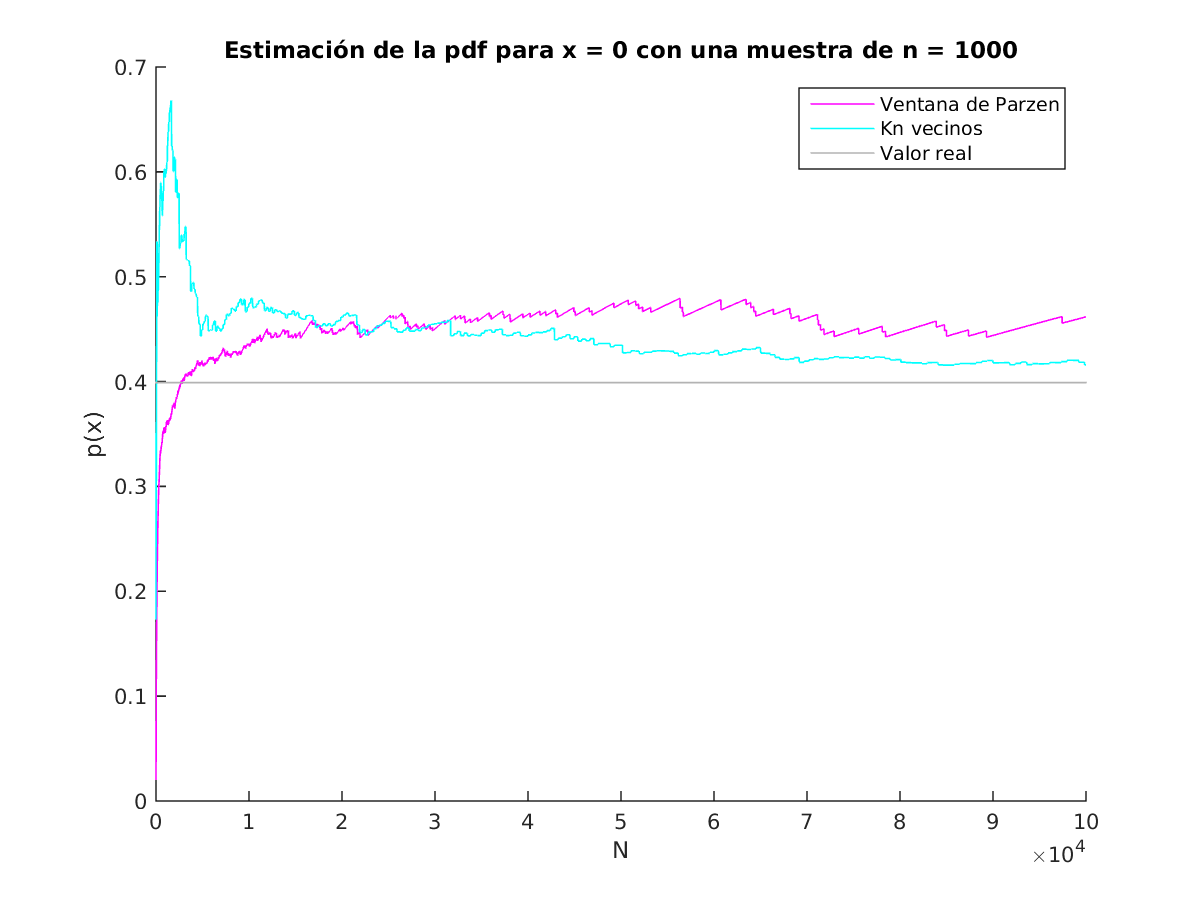
\includegraphics[width=120mm]{img/tp3/ej1-1.png}
\caption{Convergencia de la fdp de una dist. Normal (1,0).}
\end{figure}

\begin{figure}[ht!]
\centering
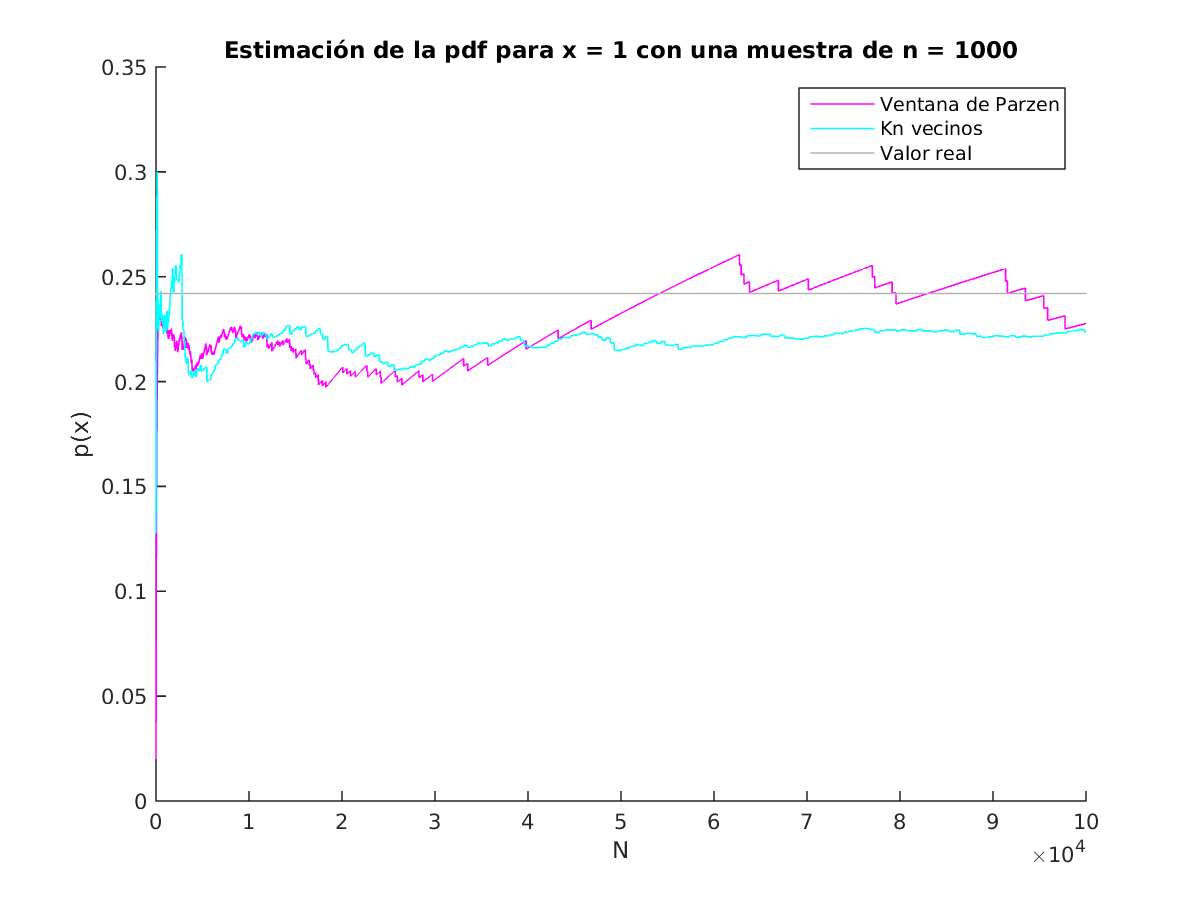
\includegraphics[width=120mm]{img/tp3/ej1-2.png}
\caption{Convergencia de la fdp de una dist. Normal (1,0).}
\end{figure}

\begin{figure}[ht!]
\centering
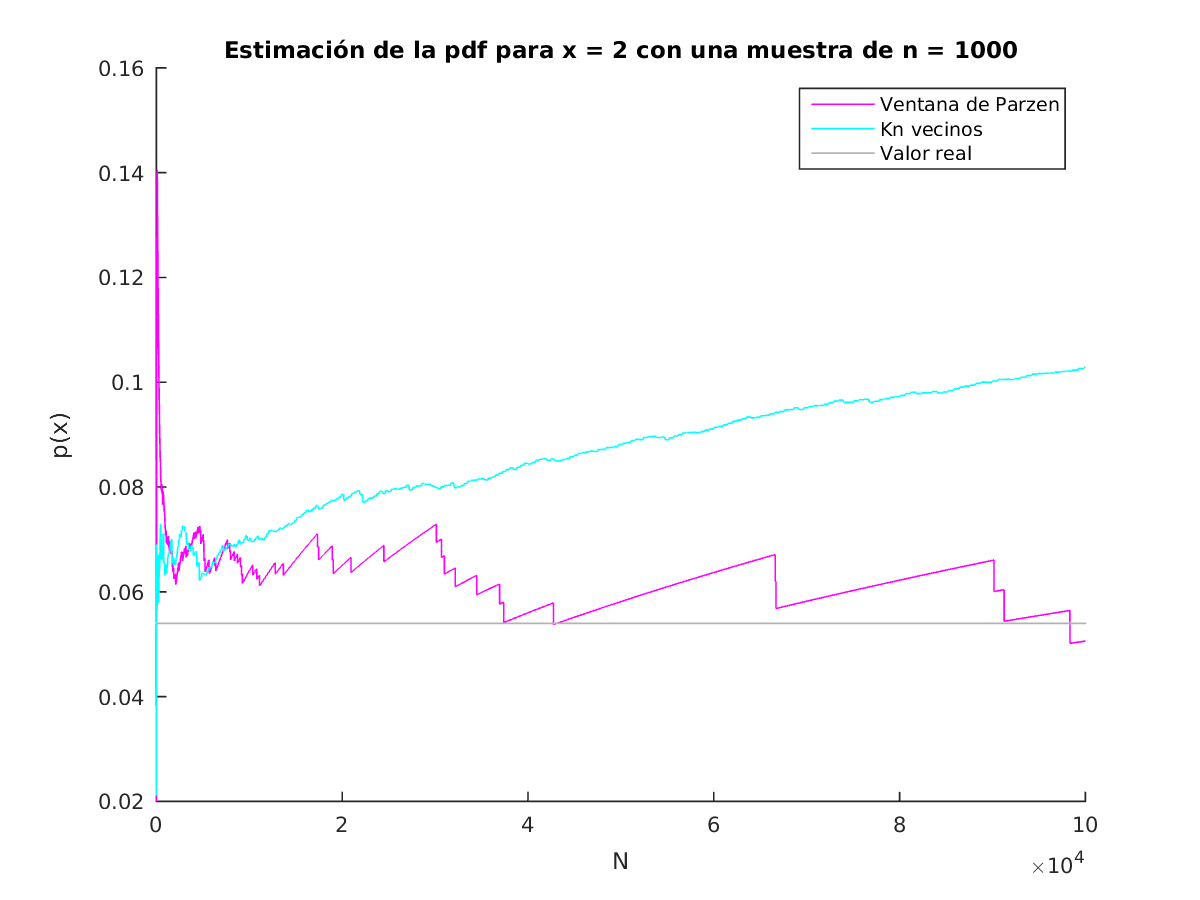
\includegraphics[width=120mm]{img/tp3/ej1-3.png}
\caption{Convergencia de la fdp de una dist. Normal (1,0).}
\end{figure}

\subsection{Ejercicio 2}

En este ejercicio se generaron datos pertenecientes a dos clases $w_1$ y $w_2$, generados a partir de dos Gaussinas bivariadas. Utilizando los métodos mencionados en el ejercicio anterior, adaptados a dos variables, se realizó la partición del espacio de características resultante (dado por las muestras generadas). Para graficar las particiones, se determinaron intervalos bidimensionales rectangulares de tamaño $1x1$ y se evaluaron los centros de cada intervalo para aproximar la $p(x)$ correspondiente ) cada muestra.
A continuación, una comparación de los resultados obtenidos entre los métodos de ventanas de parzen (con un hipercubo de dimensión 2) y $k_nn$ vecinos más cercanos. Además incluimos una comparación usando una ventana circular centrada en el punto a evaluar. Para este último, se implementó un algoritmo de ventanas de Parzen donde el $V$ utilizado es el área del círculo resultante centrado en el $x$ correspondiente, con el radio del círculo ingresado por parámetro. (ver código de función \texttt{parzenr2\_circulo}.

\subsubsection{Resultados e Imágenes}

\begin{figure}
\begin{minipage}{\textwidth}
    \begin{center}
        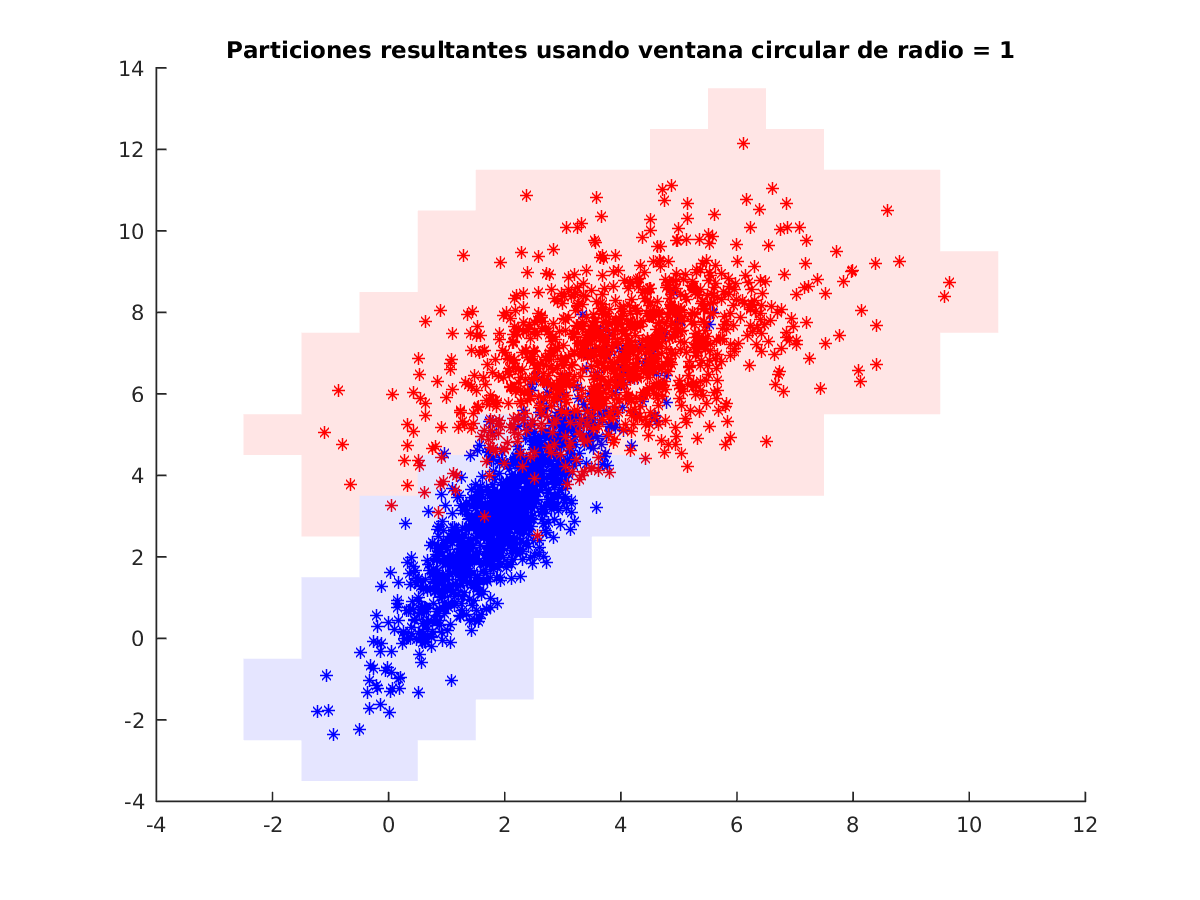
\includegraphics[width=0.4\textwidth]{img/tp3/ej2-1.png}
        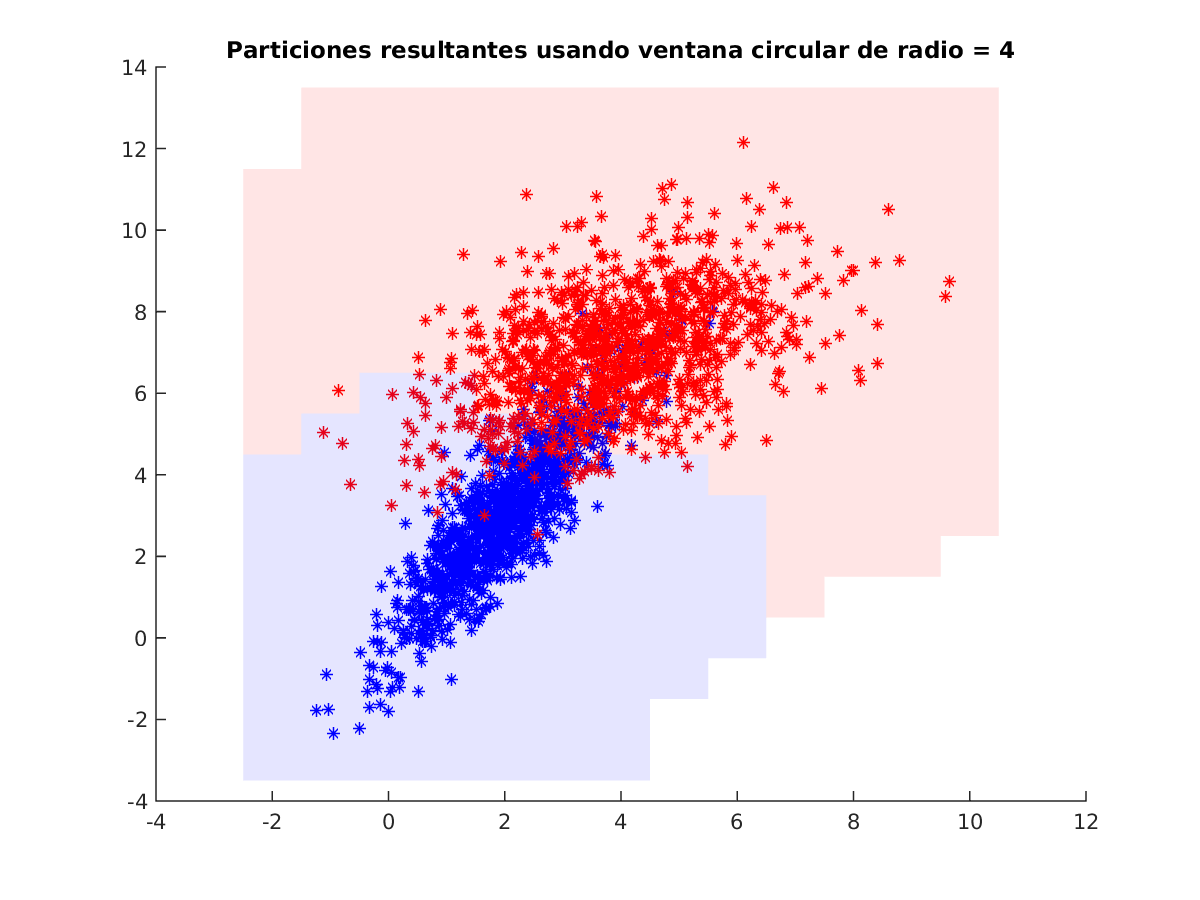
\includegraphics[width=0.4\textwidth]{img/tp3/ej2-3.png}
    \end{center}
\label{minipage:ej2-A}
\end{minipage}
\caption{\footnotesize{División del espacio de características resultante usando ventanas circulares.}} 
\end{figure}

\begin{figure}
\begin{minipage}{\textwidth}
    \begin{center}
        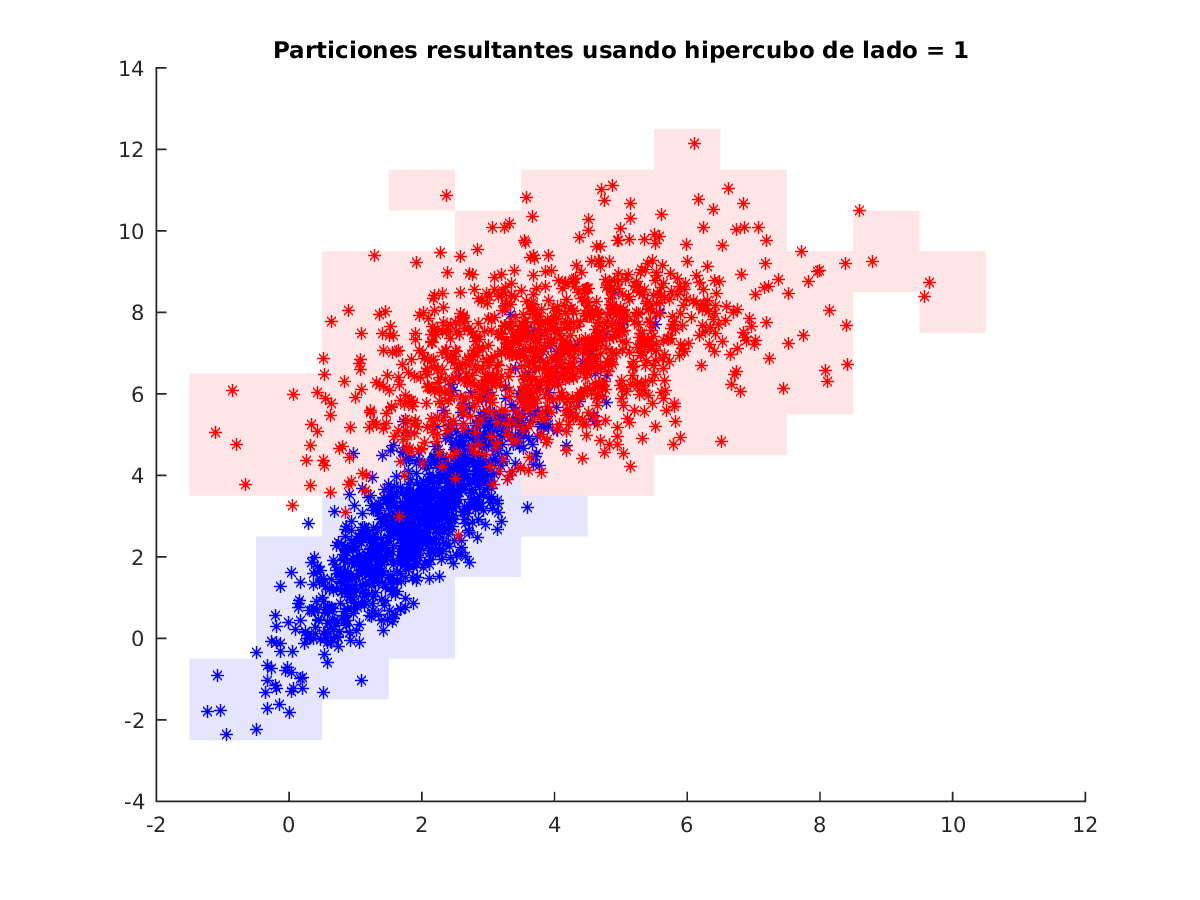
\includegraphics[width=0.4\textwidth]{img/tp3/ej2-2.png}
        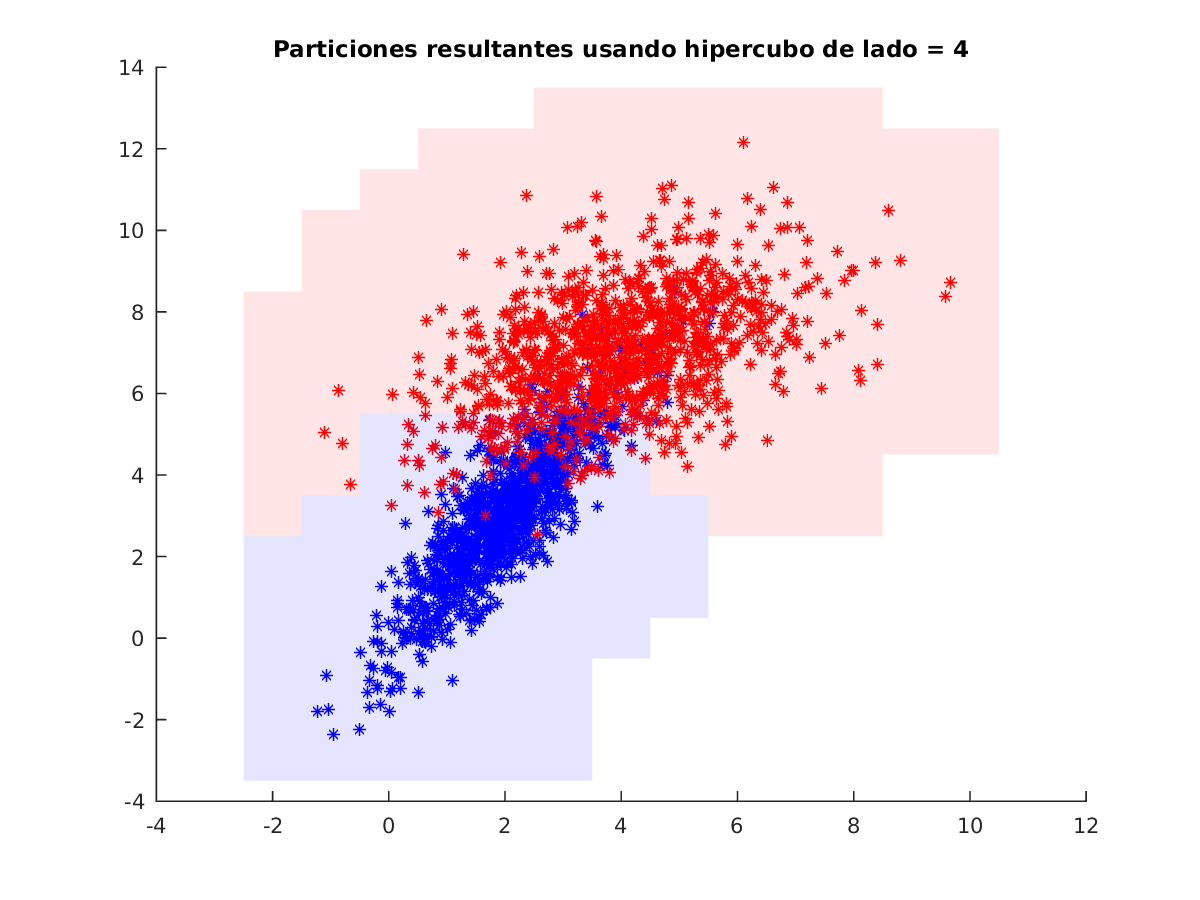
\includegraphics[width=0.4\textwidth]{img/tp3/ej2-4.png}
    \end{center}
\label{minipage:ej2-B}
\end{minipage}
\caption{\footnotesize{División del espacio de características resultante usando ventanas hipercúbicas.}} 
\end{figure}

\begin{figure}[ht!]
\centering
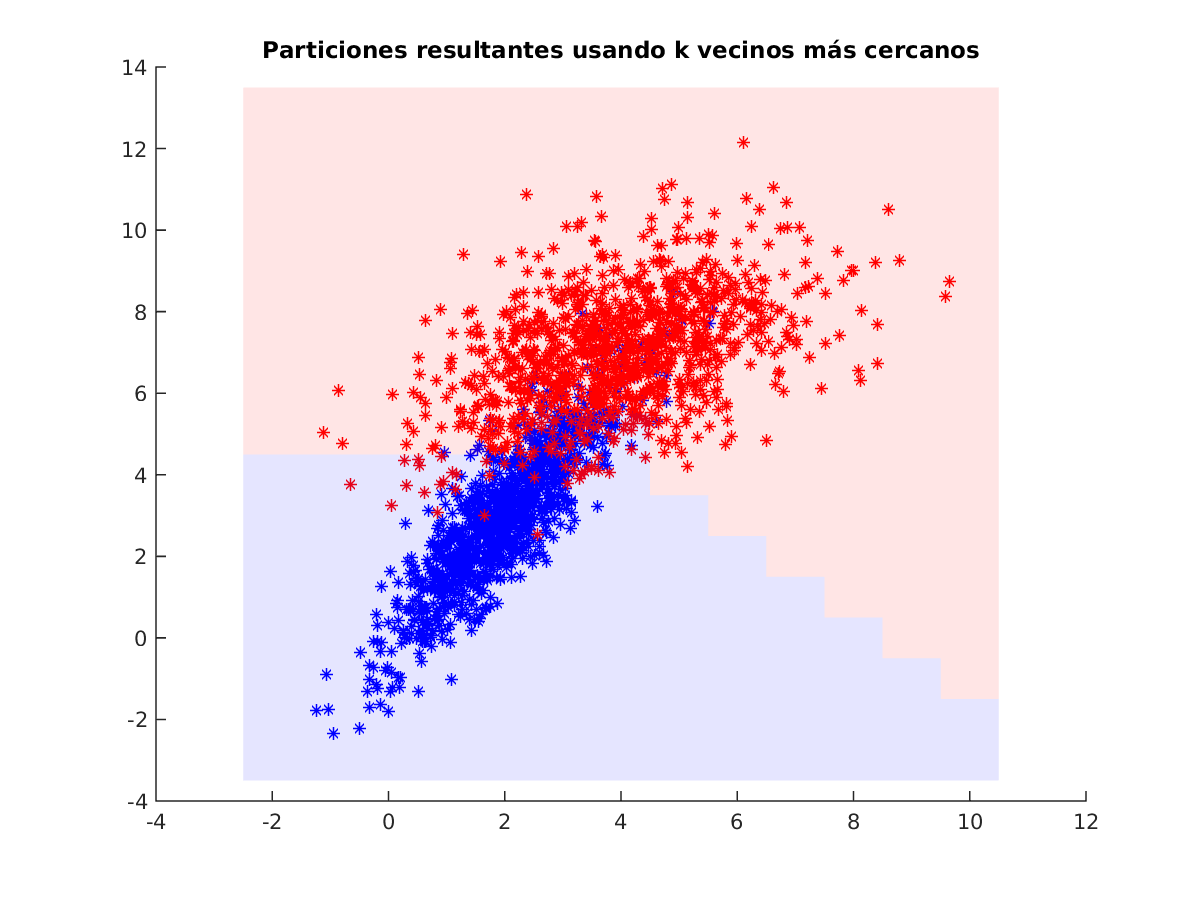
\includegraphics[width=120mm]{img/tp3/ej2-5.png}
\caption{\footnotesize{División del espacio de características resultante usando kvecinos más cercanos.}} 
\end{figure}

Uno de los problemas característicos de este método consiste en encontrar la secuencia de volúmenes $V_i$ o el tamaño de ventana óptimo. Por ejemplo, tomando $V_N$ = $V_1 / N$, los resultados son sensibles a la elección del volumen inicial $V_1$. Si el volumen inicial es muy pequeño, la mayoría de los volúmenes estarán vacíos, y la estimación de $p_n$ se vuelve muy sensible a errores (ver figura ...). Por otro lado, tomando $V_1$ grande, las variaciones en $p(x)$ que caen dentro de la misma ventana se perderán (ver figura ...). Para solucionar este problema, se presenta el siguiente método.
